\section{Implementazione}
Uno degli obiettivi principali del progetto \emph{PathS} è di fornire indicazioni di navigazione ai suoi utenti. Si è quindi presentata la necessità di dover rispondere a quesiti di \emph{routing} utilizzando le informazioni raccolte tramite le operazioni di campionamento e l'interrogazione del servizio di cartografia. 

Allo scopo di agevolare l'implementazione del componente e di ottimizare le operazioni di calcolo è stata selezionata per l'utilizzo la libreria \emph{PGRouting} la quale fornisce un grande supporto in questo senso. Questa estensione si appoggia alle funzioni \emph{GIS} del database, introducendo le capacità di calcolo del percorso tramite l'utilizzo di algoritmi generici già implementati e configurabili ad esempio Floyd-Warshall, Shortest Path A*, Dijkstra e \emph{Traveling Sales Person}.

Tuttavia per poter operare correttamente la libreria necessita che siano verificate alcune precondizioni sulla base dati da utilizzare, in particolare:
\begin{itemize}
	\item la rete di trasporto deve contenere informazioni corrette in corrispondenza delle intersezioni e degli estremi dei tratti adiacenti;
	\item la base dati deve contenere le informazioni sulla topologia della rete affinché si possa costruire un grafo utilizzabile dagli algoritmi.
\end{itemize}

Per affrontare il primo problema, la libreria mette a disposizione una funzione di ``\emph{noding}''. Tale procedura riceve in input la tabella in cui sono contenuti i dati geografici e un valore di tolleranza, quindi rielabora le informazioni cercando di rimuovere situazioni non coerenti ad esempio:
\begin{itemize}
 \item intersezioni non gestite come il caso \emph{(1)} in figura \ref{fig:pgrouting-noding}. In alcuni casi i segmenti presenti nel database potrebbero intersecarsi senza però che sia presente il corrispondente punto di intersezione. In questa situazione le successive operazioni di \emph{routing} non sarebbero in grado di sfruttare l'intersezione come punto di svolta. La procedura quindi analizza i dati \emph{GIS} per individuare le possibili sovrapposizioni e in corrispondenza delle stesse crea dei vertici aggiuntivi spezzando i segmenti. La procedura mantiene traccia del numero e dell'ordine in cui vengono decomposti gli elementi originali.
 \item segmenti adiacenti con estremi che non coincidono come il caso \emph{(2)} in figura \ref{fig:pgrouting-noding}. In questa situazione la funzione cerca di semplificare e riunire in un unico vertice gli elementi che sono all'interno della distnza di tolleranza impostata. Senza questa elaborazione i due segmenti nn potrebbero essere utilizzati dall'algoritmo di \emph{routing} dato che non sono comunicanti.
\end{itemize}

\begin{figure}[ht]
  \centering
  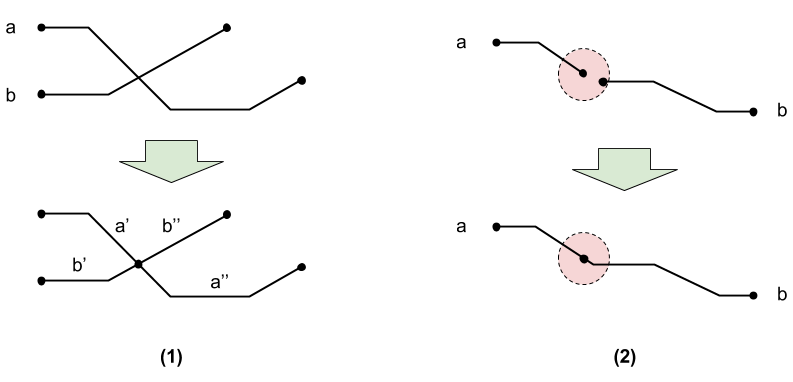
\includegraphics[width=.8\textwidth]{pgrouting-noding}
  \caption{\footnotesize{Casi in cui si applica la procedura di \emph{noding}.}}
  \label{fig:pgrouting-noding}
\end{figure}

Nel caso del database di \emph{PathS} la procedura di \emph{noding} viene eseguita sulla tabella \texttt{roadsegment} e il risultato è salvato nella tabella \texttt{roadsegment\_noded}. La procedura non altera i dati originali, ma è necessario rilanciarla ogni volta che si aggiungono nuovi elementi all'insieme dei segmenti importati tramite il servizio di cartografia.

Le informazioni dei segmenti rielaborate tramite la procedura di \emph{noding} possono essere quindi utilizzate per generare il grafo della rete di trasporto, sul quale saranno lanciati gli algoritmi di routing. L'operazione di generazione del grafo è implementata da un'altra funzione messa a disposizione dalla libreria, ovvero: \texttt{pgr\_createTopology}. In modo simile alla precedente, la funzione riceve come argomenti il nome della tabella da cui leggere le informazioni geografiche dei segmenti e un valore di tolleranza entro il quale eseguire l'operazione di unificazione dei tratti non connessi. Il risultato, nel caso specifico, porta alla generazione della tabella \texttt{roadsegment\_noded\_vertices\_pgr}. 

La struttura della tabella utilizzata per la persistenza delle informazioni dei segmenti e le conseguenti elaborazioni è presentata in figura \ref{fig:db-segments}.
\begin{figure}[ht]
  \centering
  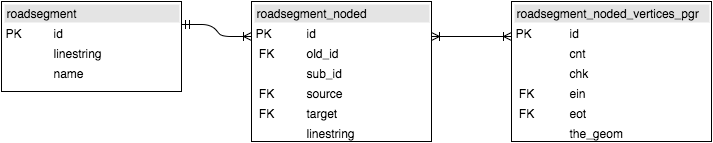
\includegraphics[width=\textwidth]{db-segments}
  \caption{\footnotesize{Schema tabelle relative ai segmenti della rete di tasporto.}}
  \label{fig:db-segments}
\end{figure}

Eseguite le operazioni di pre-processamento, i dati a sistema sono nella forma corretta per poter essere utilizzati dagli algoritmi di routing della libreria \emph{PGrouting}. A supporto dell'utilizzo e interpretazione del risultato è stata implementata la classe \texttt{app.utils.RouteResult} e le operazioni da eseguire sono state riunite nel metodo \texttt{getRouteResultFromQueryResult()}.

\section{Percorsi calcolati}
\subsection{Shortest Path}
La prima tipologia di percorso che si è deciso di calcolare è stato il caso semplice del percorso più breve (\emph{Shortest Path}). In questo modo è stato possibile valutare l'effettiva funzionalità della libreria e correggere eventuali errori nella procedura.
L'algoritmo adottato per il calcolo è quello di \emph{Dijkstra} implementato dalla funzione \texttt{pgr\_dijkstra}. Le modalità richieste per l'invocazione dell0algoritmo richiedono come argomenti:
\begin{itemize}
\item il nodo sorgente da cui inizia il percorso, specificato tramite \emph{id} così come è presente nella tabella dei vertici;
\item il nodo destinazione del tragitto, anch'esso individuato tramite \emph{id};
\item una \emph{query} con la quale ricavare i costi per ciascun arco del grafo della rete di trasporto.
\end{itemize}
Per identificare i nodi sorgente e destinazione, il server esegue una ricerca a database calcolando i vertici più vicini rispetto alle coordinate di latitudine e longitudine fornite. 

Per quanto riguarda il costo da fornire per ciascun arco, trattandosi del semplice caso \emph{Shortest Path}, si è utilizzata una \emph{query} che ritorna come peso la lunghezza in metri del segmento stesso. L'algoritmo di \emph{routing} cercherà quindi di minimizzare il peso degli archi selezionati e quindi il tragitto più breve.

Il risultato dell'interrogazione è manipolato tramite la classe di utilità \texttt{RouteResult} per ricavare alcune informazioni aggiuntive come ad esempio la lunghezza totale del percorso o le indicazioni di svolta tra un un tratto di strada e il successivo. 

Il modo in cui si presentano i dati all'applicazione client ma anche al browser web è stato scelto coerente con le altri \emph{API}. Anche in questo caso si è optato per una risposta in formato \emph{GeoJSON} ed un esempio di invocazione è riportato in \ref{response-routing}.

L'interpretazione della stessa risposta avviene con modalità diverse nei sistemi client, ovvero:
\begin{itemize}
\item nella applicazione mobile viene attivata la modalità di navigazione e le indicazioni \emph{turn-by-turn};
\item nel browser si presenta il percorso completo sulla vista mappa segnalando la lunghezza totale e un riassunto delle indicazioni di svolta.
\end{itemize}

\subsection{Percorsi con \emph{label}}
Calcolo dei percorsi valutando le label di luminosità e rumorosità. 
Viste e funzioni di supporto sul database. 
Modalità di calcolo dei costi, spiegazione delle formule.Requisiti del servizio di routing. 
\subsection{Servizio Map Quest}
Interrogazione del servizio Map Quest come riscontro e \emph{fallback}. 